
% lmao welcome to overkill land
% all because yudong wants to draw a block diagram
\ExplSyntaxOn
\NewDocumentCommand{\dopininparse}{m m}{
	\node [right, font=\scriptsize] at (\str_use:N\chipname.bpin~ \int_eval:n{#1 + 1}) {\hspace{0.5mm}\texttt{#2}};
	\draw (\str_use:N\chipname.pin~ \int_eval:n{#1 + 1}) node[inputarrow,right]{};
	\coordinate(\str_use:N\chipname-i#1) at (\str_use:N\chipname.pin~ \int_eval:n{#1 + 1});
}
\NewDocumentCommand{\dopinoutparse}{m m}{
	\node [left=-0.5mm, font=\scriptsize] at (\str_use:N\chipname.bpin~ \int_eval:n{\numpins - #1}) {\texttt{#2}};
	\draw (\str_use:N\chipname.pin~ \int_eval:n{\numpins - #1}) node[inputarrow,right]{};
	\coordinate (\str_use:N\chipname-o#1) at (\str_use:N\chipname.pin~ \int_eval:n{\numpins - #1});
}

% position, pins count, node name, label, input pins, output pins, optional args.
\NewDocumentCommand{\drawchip}{ m m m m m m O{} }{%
	\draw #1 node[dipchip, hide~ numbers, no~ topmark, anchor=pin~ 1, num~ pins=#3, #7](#2){};
	\node [above, font=\small] at (#2.north) {\texttt{#4}};

	\str_clear_new:N \chipname
	\str_set:Nn \chipname {#2}

	\int_zero_new:N \numpins
	\int_set:Nn \numpins {#3}

	\keyval_parse:NNn{\use_none:n}{\dopininparse}{#5}
	\keyval_parse:NNn{\use_none:n}{\dopinoutparse}{#6}
}

\def\splicept{coordinate(splpt){}node[splicept]{}}
\ExplSyntaxOff

\tikzset{
	splicewire/.style 2 args={
		midway,fill=white,inner sep=-0.5mm,outer sep=0mm,
		node contents={\scriptsize\texttt{[#1:#2]}}
	},
	splicept/.style={ coordinate, diamondpole, circuitikz/bipoles/length=20mm },
	splitpt/.style ={ circ },
	openwire/.style={ line width=0.2mm, ocirc, circuitikz/bipoles/length=25mm },
	circuitikz/nodes width=0.025,
	circuitikz/multipoles/thickness=1.5,
	circuitikz/multipoles/dipchip/width=1.4,
	circuitikz/multipoles/external pins width=0,
	circuitikz/multipoles/dipchip/pin spacing=0.25,
	circuitikz/multipoles/external pins thickness=0
}


\section{Super Strong TeleVision}

	With the obvious hints in the challenge statement, we got to work decoding.

	SSTV, or Slow Scan Television, is a picture transmission method used mainly by amateur radio operators to transmit and receive static pictures
	via radio in monochrome or colour\footnote{\url{en.wikipedia.org/wiki/Slow-scan_television}}. It can also be used to hide easter\footnote{
	\url{https://wiki.kerbalspaceprogram.com/wiki/List_of_easter_eggs}} eggs\footnote{\url{https://half-life.fandom.com/wiki/Portal_ARG}}...

	\subsection{Solution}

		% https://www.chonky.net/hamradio/decoding-sstv-from-a-file-on-a-linux-system
		Using \itl{PulseAudio} was used as a link between \itl{VLC} and
		\itl{QSSTV}\footnote{\url{http://users.telenet.be/on4qz/qsstv/index.html}} (an open-source Linux SSTV application), we were able to decode
		the SSTV image.

		\begin{figure}[!htbp]
			\centering
			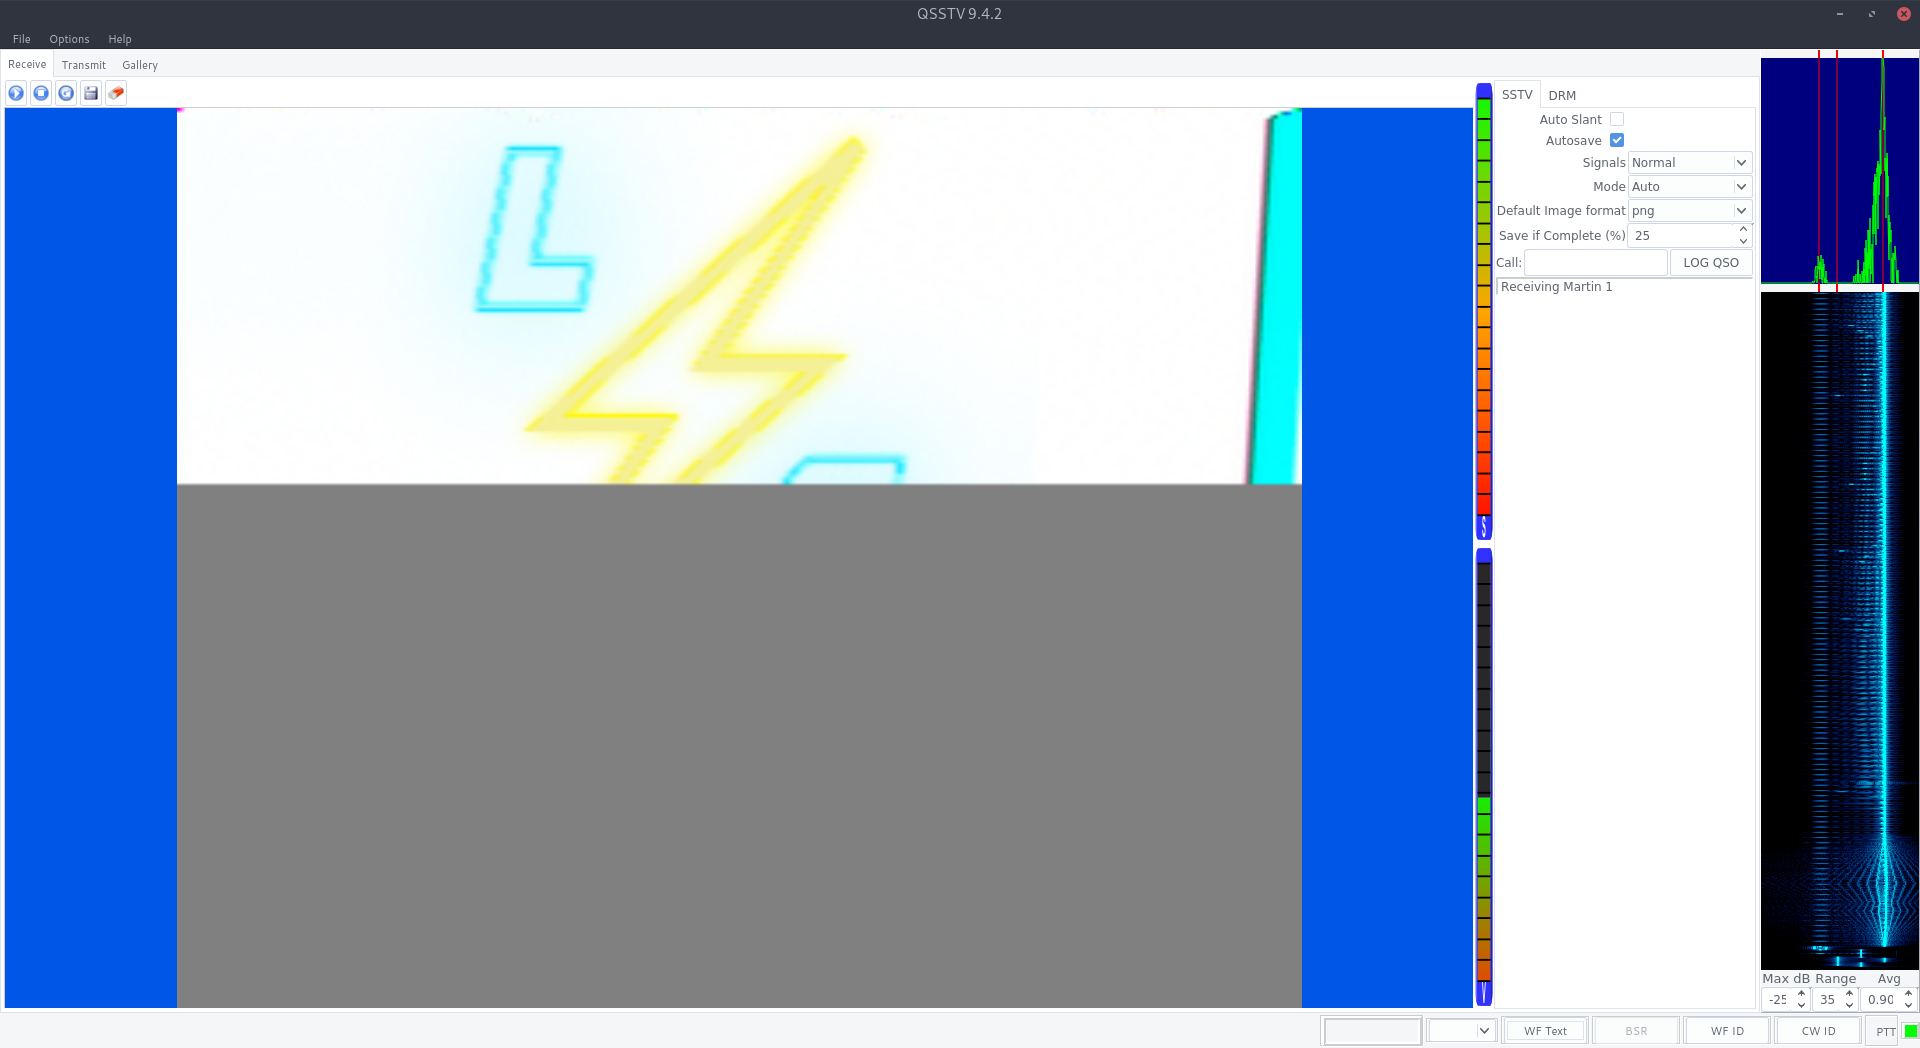
\includegraphics[width=150mm]{figures/sstv/QSSTV.png} \vspace{5mm}
			\caption{QSSTV decoding the image; its frequency spectrum can be seen on the right}
		\end{figure}


		\pagebreak
		In this case, \itl{PulseAudio} acts as the pipe that redirects the \ttt{.wav} file as an input into the decoder. To achieve that, we first
		set up a virtual \itl{null sink} and configure the system in the following manner:

		\begin{figure}[!htbp]\centering
			\begin{circuitikz}
				\drawchip{(1, 0)}{vlc}{6}{VLC}{
					1=\empty}{1=\empty
				}[circuitikz/multipoles/dipchip/width=1]

				\drawchip{(4, 0)}{pulseaudio}{6}{PulseAudio}{
					1=\empty}{1=\empty
				}[circuitikz/multipoles/dipchip/width=1]

				\drawchip{(7, 0)}{qsstv}{6}{QSSTV}{
					1=\empty}{1=\empty
				}[circuitikz/multipoles/dipchip/width=1]

				% draw backwards...
				\draw[line width=.4mm] (vlc-i1) -- ++(-1, 0) node[anchor=mid east]{.wav file} {};
				\draw[line width=.4mm] (vlc-o1) -- (pulseaudio-i1) {};
				\draw[line width=.4mm] (pulseaudio-o1) -- (qsstv-i1) {};
				\draw[line width=.4mm] (qsstv-o1) -- ++(1.2, 0) node[anchor=west,inputarrow]{} ++(.1,0) node[anchor=mid west]{image} {};


			\end{circuitikz}\vspace{5mm}
			\caption{Data Pipeline Setup}
		\end{figure}

	% end subsection

	\subsection{Flag}
		After some suspense as the SSTV audio played back in real time, the image was fully decoded, revealing the flag, which
		was \cddcflag{Light\$peedCorp-\$\$TV}.

		\begin{figure}[!htbp]\centering
			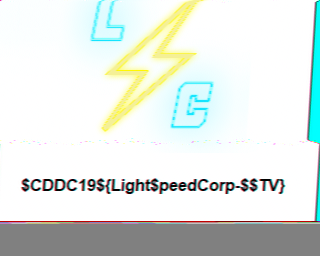
\includegraphics[width=80mm]{figures/sstv/SSTV.png} \vspace{5mm}
			\caption{Decoded SSTV Image}
		\end{figure}
	% end subsection
% end section
